\documentclass{report}
\usepackage[utf8]{inputenc}
\usepackage{graphicx}
\usepackage{sidecap}
\usepackage{fancyhdr}
\usepackage{lscape}
\usepackage[absolute]{textpos}
\usepackage{SIunits}
\usepackage{sistyle}
\usepackage{amsmath}

\makeatletter
\def\maketitle{%
  \null
  \thispagestyle{empty}%
  \vfill
  \begin{center}\leavevmode
    \normalfont
    {\LARGE \@title\par}%
    \vskip 1cm
    {\Large \@author\par}%
    \vskip 1cm
    {\Large \@date\par}%
  \end{center}%
  \vfill
  \null
  \newpage
  }
\makeatother
\author{Groupe : Mattens Simon, Dom Eduardo\\ BAB2 Sciences Informatiques}
\title{Rapport : circuits RC et RL}
\date{19 avril 2018}

\begin{document}
\maketitle

\section*{1 Introduction}
\hspace*{0.5cm}
Le but de la manipulation est l'étude de la charge et la décharge d’un
condensateur C à travers une  résistance  R  ainsi  que  la  vérification expérimentale  de  la  loi d'association  de  capacités. 
La manipulation comportera également l’étude d’un circuit RL à constante de temps courte.

\section*{2 R\'esum\'e th\'eorique}
\subsection*{2.1 Condensateur}
\hspace*{0.5cm}
Un condensateur est formé de 2 conducteurs isolés électriquement l'un de l'autre, donc séparés par un diélectrique. Les 2 conducteurs sont en influence totale (toute ligne de champ issue de l'un aboutit sur l'autre), les surfaces en regard portant des charges opposées.
\begin{figure}[ht!]
\centering
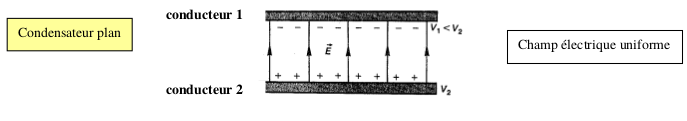
\includegraphics[width=90mm]{cond.png}
\label{overflow}
\end{figure}
\\
Un condensateur est symbolisé par 2 barres parallèle et caractérisé par une capacité C définie par la relation  : 
\begin{equation}
    Q = C\cdot U
\end{equation}
Pour un montage en parall\`ele des condensateurs, la formule est:

\begin{equation}
    C_{eq} =\sum{C_{i}}
\end{equation}

La charge d'un condensateur \`a travers une r\'esistance est donn\'ee par:
\begin{equation}
    Q(t) = Q_{0}(1-e^{\frac{-t}{\tau}})
\end{equation}

Quant \`a la d\'echarge, la formule est la suivante :
\begin{equation}
    Q(t) = Q_{0}e^{\frac{-t}{\tau}}
\end{equation}

L'unit\'e des capacit\'es est exprim\'e en Farad.

\subsection*{2.2 Bobine}
Une bobine est formée d’un fil conducteur enroulé formant des spires. à l’intérieur des spires, on trouve de l’air ou un matériau ferromagnétique. Un courant parcourt ce fil et un champ magnétique est généré par cette bobine. Lorsque des variations de courant se produisent, il y a variation du flux du champ magnétique et donc induction d’une tension électromotrice aux bornes de la
bobine, plus précisément il y a auto-induction d’une tension U tel que
: 
\begin{equation}
    U = -L\frac{dI}{dt}
\end{equation}
L'unité d'inductance est le Henry(H).
\begin{figure}[ht!]
\centering
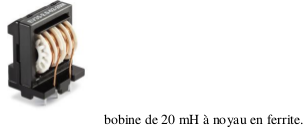
\includegraphics[width=90mm]{bobine.png}
\label{overflow}
\end{figure}
\subsection*{2.3 Résistance}
\hspace*{0.5cm}
Tout matériau est caractérisé par sa résistivité électrique $\rho$ et on distingue ainsi : \\

\begin{tabular}{|l|c|r|}
  \hline
  Conducteur & Semi-conducteur  & Isolant \\
  \hline
  $\rho <  10^{-5} \ \Omega .m $ & $10^{-5} < \rho < 10^{7} \Omega.m $ & $\rho > 10^{7} \Omega.m $\\
  \hline
\end{tabular}
\\ \\
La résistance électrique d’un élément cylindrique (longueur L et section transversale S) est donnée par $R = \frac{\rho L}{S} $ et elle va 
déterminer l'intensité du courant traversant le conducteur en fonction de la valeur de la tension appliquée à ses bornes U = RI (loi d'Ohm).
Le courant électrique I représente la quantité de charge dQ traversant une section du conducteur pendant l'intervalle de temps dt :  $I = \frac{dq}{dt} $.
\section*{3 Dispositif exp\'erimental}
\subsection*{3.1 Mat\'eriel utilis\'e}
\begin{itemize}
\item Eléments R, L et C et plaque de réalisation de circuits 
Nous disposons de  plusieurs  résistances, selfs (ou  bobines) et condensateurs à fixer sur une plaquette d'essai. 

\item Circuit RC  à longue constante de temps : carte ARDUINO + PC. L’alimentation en tension  continue(0 -5  V)  ainsi  que  le voltmètre mesurant la  tension  aux bornes du condensateur seront fournis par une carte d’acquisition ARDUINO UNO pilotée via PC.  

\item Circuits RC et RL à constante de temps courte : générateur de signaux + oscillo. Pour  les  circuits  à  constante  de  temps  rapide,  il  est  impossible  d'observer "à l'œil" la croissance  (ou  décroissance)  de  la tension  aux  bornes  du  condensateur (circuit  RC)  ou  de  la tension  aux bornes de  R  (circuit  RL).

\item Un g\'en\'erateur de tension alternative de forme carr\'ee. Celui-ci permet de stabiliser le comportement du circuit.

\item Un oscilloscope.
\end{itemize}

\section*{4 Prise des mesures \& r\'esultats}
Après avoir réalisé le  circuit via  une  plaquette  d'essai  et  une  carte d'acquisition ARDUINO, nous avons vérifié qu'on  a  bien  placé en série une  résistance  et  un  condensateur de 0.982 nF.
Par calcul, on obtient que la constante de temps du circuit  vaut 0.002
Nous avons ensuite démarré un programme sur l'arduino qui génère la tension au circuit (0-5V) et qui lit et enregistre la tension aux bornes du condensateur C
afin d'observer la variation (augmentation) de  la  tension  aux  bornes  du condensateur  qui s'enregistre  en  fonction  du  temps  toutes les  5  secondes et  les  résultats  de  mesure correspondants.
Après la charge quasi complète du condensateur , la décharge du condensateur s'enregistre automatiquement  et on observe la variation  (diminution)  de  la tension  aux  bornes  du  condensateur  qui s'enregistre en fonction du temps toutes les 5 secondes.
Ces 2 variations sont schématisé ci dessous.
\subsection*{}
\hspace*{0.5cm}
\begin{figure}[ht!]
\centering
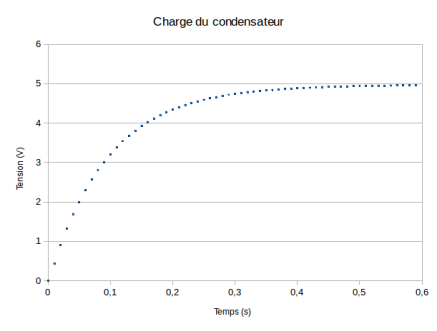
\includegraphics[width=90mm]{charge.png}
\label{overflow}
\end{figure}
On peut voir que le condensateur charge plus vite au début qu'à la fin.
La courbe tend vers 5V et y est très proche après 0.6s .
\pagebreak
\subsection*{}
\begin{figure}[ht!]
\centering
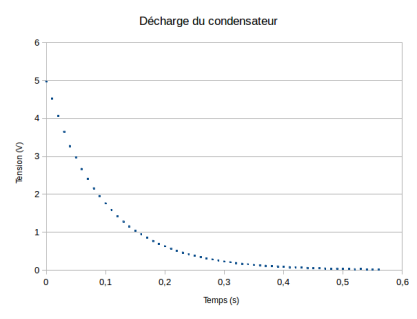
\includegraphics[width=90mm]{decharge.png}
\label{overflow}
\end{figure}
On peut voir que le condensateur décharge plus vite au début qu'à la fin.
Il faut environ 0.6s pour qu'il se décharge complètement.
\hspace*{0.5cm}
\section*{5. Analyse des r\'esultats}
Lorsque l'on superpose les courbes de charges et décharges, les courbe se coupent à la demi-vie  de la charge et de la décharge du condensateur. C’est le temps nécessaire pour que la tension aux bornes du condensateur atteigne la moitié de sa valeur maximale.
\subsection*{5.1 Analyse dimensionnelle de la constante de temps $\tau$ }
V\'erifions que $\tau$ = RC a bien des unit\'es de temps.
\\
On sait:
   $$[\tau] = 1\Omega \cdot 1F$$
Par la loi d'Ohm, on a que:
   $$[\tau] = \frac{1V \cdot 1F}{1A}$$
On sait :
   $$1F = \frac{1s \cdot 1A}{1V}$$
En conclusion,
   $$[\tau] = \frac{1V \cdot 1s \cdot 1A}{1A \cdot 1V}$$
  $$\Leftrightarrow [\tau] = 1s$$
L'unit\'e internationale du temps est bel et bien la seconde.
\subsection*{5.2 Circuit \`a constante de temps rapide}
\hspace*{0.5cm}
Nous avons réglé la fr\'equence \`a 1 kHz et choisi une forme de signal carr\'ee sur le g\'en\'erateur de signaux(GS) en tension alternative, nous avons visualis\'e cette tension sur l'oscilloscope.
L'amplitude est de 2 Volts et la p\'eriode de 0,5 seconde.
Nous avons ensuite branch\'e cette tension aux bornes du circuit RC. 
L'amplitude est toujours de 2 Volts et la p\'eriode est de 1 seconde.
Ensuite, nous avons calcul\'e exp\'erimentalement la demi-vie:
\begin{equation}
   T_{1/2} = \frac{0,3}{5}
\end{equation}
On peut maintenant calculer $\tau$:
\begin{equation}
   \tau = \frac{T_{1/2}}{ln2}
\end{equation}
\begin{equation}
   \Leftrightarrow \tau = \frac{0,3}{5 \cdot ln2} 
\end{equation}

\begin{equation}
   \Leftrightarrow \tau = 0.08656170245 \text{ seconde} 
\end{equation}
Valeur th\'eorique de $\tau$ : 0.001 seconde.
\\
Nous constatons que la valeur th\'eorique est plus petite que la valeur exp\'erimentale. D\`es lors, on doit tenir compte de la r\'esistance interne du g\'en\'erateur de signaux.
Pour calculer cette r\'esistance interne, nous savons que :
\begin{equation}
   R = \frac{\tau}{C} 
\end{equation}
\begin{equation}
  \Leftrightarrow R = \frac{0.08656170245}{0,1 \cdot 10^{-6}} 
\end{equation}
\begin{equation}
  \Leftrightarrow R = 865617.0245 \ohm
\end{equation}
\\ On ne  doit pas tenir compte de la résistance de l'oscillateur car elle est très grande.

\subsubsection*{5.2.1 Capacit\'es mont\'ees en s\'erie}
\hspace*{0.5cm}
Nous avons remplac\'e la capacit\'e par 2 capacit\'es en s\'erie. Nous avons observé la d\'echarge. Nous avons \'egalement mesur\'e la demi-vie.
\begin{equation}
   T_{1/2} = \frac{0,2}{5}
\end{equation}

Comme les deux capacit\'es de 0,1\micro F sont mont\'ees en s\'erie, nous pouvons calculer th\'eoriquement C equivalent:

\begin{equation}
   \frac{1}{C_{eq}} =  \frac{1}{C_{1}}+\frac{1}{C_{2}}
\end{equation}

\begin{equation}
   \Leftrightarrow C_{eq} =  (\frac{1}{0,1 \cdot 10^{-6}}+\frac{1}{0,1 \cdot 10^{-6}})^{-1}
\end{equation}

\begin{equation}
   \Leftrightarrow C_{eq} = 5 \cdot 10^{-8} F
\end{equation}
\begin{equation}
   \Leftrightarrow C_{eq} = 0,05 \micro F
\end{equation}

Calculons maintenant C \'equivalent avec les valeurs empiriques.
\begin{equation}
    C_{eq} = \frac{\tau}{R}
\end{equation}
\begin{equation}
    \Leftrightarrow C_{eq} = \frac{\frac{T_{1/2}}{ln(2)}}{R}
\end{equation}
\begin{equation}
    \Leftrightarrow C_{eq} = \frac{0,2}{5 \cdot ln(2) \cdot R}
\end{equation}
\begin{equation}
    \Leftrightarrow C_{eq} = \frac{0,2}{5 \cdot ln(2) \cdot 865617.0245}
\end{equation}
\begin{equation}
    \Leftrightarrow C_{eq} = 6.66666686\cdot 10^{-8}
\end{equation}
\begin{equation}
    \Leftrightarrow C_{eq} = 0.066 \micro F
\end{equation}
Nous constatons que la diff\'erence de valeur entre C \'equivalent calcul\'e avec les valeurs empiriques et l'autre sont sensiblement proches. En effet, il n'y a que 0,016 \micro F de diff\'erence.
\subsection*{5.2.2 Capacit\'es mont\'ees en parall\`eles}
\hspace*{0.5cm}
Nous avons remplac\'e la capacit\'e par 2 capacit\'es en parall\`eles. Nous avons observé la d\'echarge. Nous avons \'egalement mesur\'e la demi-vie.
\begin{equation}
   T_{1/2} = \frac{0,6}{5}
\end{equation}
Comme les deux capacit\'es de 0,1\micro F sont mont\'ees en parall\`eles, nous pouvons calculer th\'eoriquement C equivalent:
\begin{equation}
    C_{eq} = C_1 + C_2
\end{equation}
\begin{equation}
    C_{eq} = 0,1 \cdot 10^{-6} +  0,1 \cdot 10^{-6}
\end{equation}
\begin{equation}
    C_{eq} = 2 \cdot 10^{-7}
\end{equation}
\begin{equation}
    C_{eq} = 0,2 \micro F
\end{equation}

Calculons maintenant C \'equivalent avec les valeurs empiriques.
\begin{equation}
    C_{eq} = \frac{\tau}{R}
\end{equation}
\begin{equation}
    \Leftrightarrow C_{eq} = \frac{\frac{T_{1/2}}{ln(2)}}{R}
\end{equation}
\begin{equation}
    \Leftrightarrow C_{eq} = \frac{0,6}{5 \cdot ln(2) \cdot R}
\end{equation}
\begin{equation}
    \Leftrightarrow C_{eq} = \frac{0,6}{5 \cdot ln(2) \cdot 865617.0245}
\end{equation}
\begin{equation}
    \Leftrightarrow C_{eq} = 2 \cdot 10^{-7}
\end{equation}
\begin{equation}
    \Leftrightarrow C_{eq} = 0,2 \micro F
\end{equation}
On constate que la valeur de C calcul\'e empiriquement est \'egale \`a la valeur de C calcul\'e th\'eoriquement.

\section*{6 Conclusion}
\hspace*{0.5cm}
Nous avons \'etudi\'e la charge et la d\'echarge  d'un condensateur C \`a travers une r\'esistance R . On a aussi v\'erifi\'e la loi exp\'erimentale de la loi d'association de capacit\'es en s\'erie et en parall\`ele.\\

\end{document}